\documentclass[aps,rmp,twocolumn,amsmath,amssymb,nofootinbib,superscriptaddress]{revtex4}

\newcommand{\bra}[1]{\langle#1|}
\newcommand{\ket}[1]{|#1\rangle}
\newcommand{\op}[2]{\hat{\textbf{#1}}_{#2}}
\newcommand{\dagop}[2]{\hat{\textbf{#1}}_{#2}^\dag}
\usepackage[pdftex]{graphicx}
\usepackage{mathrsfs}
\usepackage[colorlinks]{hyperref}
\usepackage[dvipsnames]{xcolor}

\newcommand{\sihui}[1]{{\color{Orchid}{#1}}}
\newcommand{\peter}[1]{{\color{YellowGreen}{#1}}}
\newcommand{\comment}[1]{{\color{blue}{#1}}}
\newcommand{\ah}{\hat{a}}
\newcommand{\adagh}{\hat{a}^\dag}

\begin{document}

\bibliographystyle{apsrev}

%
% Title
%

\title{The Resurgence of the Linear Optics Interferometer --- Recent Advances \& Applications}

%
% Authors
%

\author{Si-Hui Tan}
\email[]{sihui\_tan@sutd.edu.sg}
\affiliation{Singapore University of Technology and Design, 8 Somapah Road, Singapore}

\author{Peter P. Rohde}
\email[]{dr.rohde@gmail.com}
\homepage{http://www.peterrohde.org}
\affiliation{Centre for Quantum Software \& Information (CQSI), Faculty of Engineering \& Information Technology, University of Technology Sydney, NSW 2007, Australia}

\date{\today}

\frenchspacing

%
% Abstract
%

\begin{abstract}
\end{abstract}

\maketitle

\tableofcontents

\section{Introduction}

\comment{To do}

Technical advancements have been made on many fronts. It is possible now to put single-photon sources and linear-optical networks on a silica chip. The advantage of using such integrated photonics over bulk optics is that it is more stable against phase fluctuations, and miniaturized. This increases the scalability of optical implementations of quantum information protocols.

\section{Mathematical background}

A idealized single photon in a quantum interferometer is described by its creation operator $\adagh_{j}$, where $j$ is the label of the mode the photon is in  within the interferometer. The creation and annihilation operators satisfy the bosonic comutation relationship $[\ah_{j},\adagh_{k}]=\delta_{j,k}$. A similar commutation relationship can be written when additional degrees of freedom, such as polarization, orbital angular momentum, and time-bins \cite{bib:Tillmann2015,bib:Bozinovic2013, bib:Nicolas2014, bib:Humphreys2013, bib:Donohue2013}, are present. When multiple photons are present, they experience quantum interference when all quantum labels are the same.

The action of a $2d$-port linear optical interferometer (with an equal number of input and output ports) is expressed as an application of unitary operations on the creation operators,

\begin{align}
b_i^{\dag}=\sum_{j=1}^d U_{ij}a_j^\dag \ ,
\end{align}
where $a_j^\dag$ and $b_i^\dag$ are the creation operators of a single input and output photon in the $j$-th and $i$-th modes respectively, and $U\in SU(d)$. All such transformations can be expressed as sequences of beamsplitters and phase-shifters \cite{bib:Reck1994}. In the case when photons have additional labels, for instance, if they have internal labels on top of spatial labels, it is also possible to derive an analogous decomposition, known as a cosine-sine decomposition \cite{bib:Dhand2015}, that realizes the unitary transformation on the photons as a sequence of beamsplitters and internal transformations. Toolkits using group theory are being developed to deal with partial distinguishabilities among interfering photons \cite{bib:Tan2013,bib:deGuise2014,bib:deGuise2015}. Others use quantum-to-classical transitions to explain multiparticle interference \cite{bib:Ra2013}. \sihui{Experimental implementation [Walmsley, Jennewein]}

\section{Optical encoding of quantum information on single-photons}

Using quantum states of light, there are a multitude of approaches to encoding quantum information. Beginning with a logical qubit,
\begin{align}
\ket\psi_L = \alpha \ket{0}_L + \beta\ket{1}_L,
\end{align}
we now discuss the most prominent such encodings, which have been widely employed. We will specifically focus on single-photon encodings, as opposed to, for example, continuous variable encodings.

These encodings are all isomorphic to one another, but nonetheless, because they are represented using entirely different physical systems, they each exhibit their own unique advantages and disadvantages, and methods by which to implement operations upon them.

%\subsection{Single-photons}

\subsubsection{Polarisation}

In polarisation encoding, the polarisation of a single photon in a single spatial mode encodes a logical qubit. Specifically, we represent the logical qubit as,
\begin{align}
\ket\psi_L = \alpha\ket{H} + \beta\ket{V},	
\end{align}
where $H$ ($V$) denotes a horizontally (vertically) polarised single photon.

Polarisation encoding has the elegance that the most common optical error mechanisms, such as loss or path-length mismatch, affect the two logical basis states equally. Furthermore, single-qubit operations may be directly implemented using wave-plates, which implement a rotation in polarisation space. Relevant to the preparation of large entangled states, such as cluster states, polarising beamsplitters can be employed to perform non-deterministic Bell state projections.

When physically constructing protocols based on polarisation-encoding, for obvious reasons it is extremely important that optical components be polarisation-preserving. Not doing so would obviously corrupt the logical state. Some waveguide technologies, for example, exhibit different refractive indices for the two polarisations.

\subsubsection{Dual-rail}

In dual-rail encoding, a single photon encodes a logical qubit as a superposition across two spatial modes,
\begin{align}
\ket\psi_L = \alpha\ket{1,0} + \beta\ket{0,1},
\end{align}
where $\ket{i,j}$ is a two-mode state with $i$ ($j$) photons in the first (second) spatial mode. Using this encoding, phase-shifters and beamsplitters between the two spatial modes implement arbitrary single-qubit operations. Unfortunately, because the two basis states evolve via independent paths, our dual-rail qubits are susceptible to path-length-mismatch, a problem that does not affect polarisation encoding.

Converting between polarisation- and dual-rail-encoding is trivial using polarising beamsplitters, which separate horizontal and vertical components into distinct spatial modes, or vice-versa.

\subsubsection{Time-bins}

Time-bin qubits encode quantum information into the time-of-arrival of single photons, which have fixed polarisation and reside in a single spatial mode. Effectively, we discretise the direction of propagation of photons into discrete bins, which are treated as orthogonal basis states. Specifically, we are employing the encoding,
\begin{align}
\ket\psi_L = \alpha\ket{1}_{t}\ket{0}_{t+\tau} + \beta \ket{0}_{t}\ket{1}_{t+\tau},
\end{align}
where $\ket{0}_t$ ($\ket{1}_t$) denotes the vacuum (single-photon) state with arrival time $t$. Here $\tau$ is the time-bin separation, which must be sufficiently large that the temporal envelopes of neighbouring photons do not overlap, thereby ensuring orthogonality of the logical basis states.

This encoding is particularly resource-savvy, since a single spatial mode (e.g length of optical fibre) can encapsulate many time-bin qubits as a `time-bin-train'. The amount of quantum information that can be encoded into the train is limited only by its physical length.

Unlike polarisation or dual-rail encoding, time-bin encoding does not lend itself to `native' single-qubit operations. Rather, fast switching can be used to spatially separate neighbouring time-bins, implement a beamsplitter operation between them, before converting back to time-bin encoding.

Time-bin encoding was first conceived via a single-photon passing through a Mach-Zedner interferometer with its two paths having different lengths \cite{bib:Brendel99}. If the photon passes through the shorter (longer) path, it will arrive at the output port in an `early' (`later') time-bin labelled $\ket{e}$ ($\ket{\ell}$). Thus, the photon will exit the interferometer in a state that is a superposition of these two states. Owing to difficulties in implementing qubit operations in this basis, it was at the time mostly used for demonstrating quantum communication over long distances \cite{bib:Thew02,bib:Marcikic04}. With the advent of faster optical components, and single-photon detectors, it has become feasible to perform any single qubit operation, and a post-selected CPHASE gate on time-bin qubits \cite{bib:Humphreys2013}. These gates form an universal set for quantum computing. At the same time, an ultrafast measurement technique for recovering time-bin qubits was also demonstrated \cite{bib:Donohue2013}.

In Humphrey {\it et al.} \cite{bib:Humphreys2013}, the time-bin qubits have a polarization register which is used to toggle between the mode in which qubits are stored and transmitted, {\it i.e.} the `register' mode, and the mode in which qubits are manipulated, {\it i.e.} the `processing' mode using a polarization rotation. Other operations needed are a displacement operation, that moves a time-bin qubit in the processing polarization in time relative to other qubits, a partial polarization rotation between the register and processing polarizations to couple them, and a photon number measurement in a bin. The polarization rotation and polarization coupling operations were implemented using a fast integrated optical switch based on polarization-sensitive cross-phase modulation with a switching time of less than 10ps. The displacement was implemented using a calcite crystal of a size that is of a path-length difference equal to an integer multiple of the time-bin separation. Using these operations and post-selection using a single-photon detectors, the authors were able to perform a heralded CPHASE gate \cite{bib:KLM01}.

In Donohue {\it et al.} \cite{bib:Donohue2013}, time-bins were converted into frequency bins using a nonlinear optical process known as sum-frequency generation (SFG) by pumping them on a crystal with a laser beam. The waveforms of the input photons and the pump beam are chirped in opposite directions in frequency, so that the output is a set of two peaks separated in frequency by an amount proportional to the time separation of the time bins. The output can then be measured with detectors that are slow compared to this separation. This is unlike conventional time-bin measurements which involve sending a time-bin state through an unbalanced Mach-Zedner interferometer matched to the time-bin separation to produce three output pulses that are separated by the time delay, and then having to resolve the middle pulse in time. 

Apart from these promising advances in implementing time-bin qubit gates and ultrafast time-bin measurements, scalable networks using time-bin encoding are also possible using a loop-based architecture \cite{bib:Motes14}. This is discussed in more detail in Section \ref{sec:timebins}.

%\subsection{Continuous-variables}

%\subsubsection{Coherent states}

%\subsubsection{Squeezed states}

\section{Efficient circuit decompositions of linear optics networks}

The task of implementing an arbitrary quantum computation on linear optics comes down to implementing an arbitrary $n\times n$ unitary matrix. If a non-unitary transformation is desired, it can be embedded within a unitary matrix with larger dimensions. An algorithm for expressing an arbitrary unitary matrix {\it exactly} in terms of a sequence of beamsplitters and phase-shifters was described by Reck \emph{et al.} \cite{bib:Reck1994}. This decomposition requires $\mathcal{O}(n^2)$ linear optical elements, and the algorithm for finding the decomposition has polynomial runtime. Thus, such decompositions can always be determined and implemented efficiently. The layout for the original Reck \emph{et al.} decomposition is shown in Fig.~\ref{fig:Reck}. However, since then a multitude of alternate decompositions have been found. A notable downside of the original decomposition is that different photons experience different circuit depth, i.e pass through different numbers of optical elements, resulting in asymmetry in losses and the accumulation of errors.

\begin{figure}[!htb]
\includegraphics[width=\columnwidth]{reck}
\caption{Efficient decomposition of arbitrary linear optics networks into a sequence of beamsplitters and phase-shifters.} \label{fig:Reck}	
\end{figure}

Alternatively, Mach-Zedner interferometers can also be employed as building blocks instead of beamsplitters and phase-shifters \cite{bib:Reck1994, bib:Englert2001}. Later, it has been shown that any nontrivial beamsplitter, that does more than permuting modes or adding phases to them, is universal for linear optics \cite{bib:Bouland2014}. However, they do not provide an explicit construction for arbitrary unitaries.

If the linear optical transformations can be realized on various degrees of freedom of light, then it is possible to realize a $n\times n$ arbitrary unitary transformation, where $n=n_s n_p$ for $n_s$ spatial modes, and $n_p$ internal modes, by a sequence of $\mathcal{O}(n_s^2 n_p)$ beamsplitters and $\mathcal{O}(n_s^2)$ internal transformations \cite{bib:Dhand2015}. Their approach reduces the required number of beamsplitters but increases the total number of optical elements needed by a factor of 2.

\section{Reconstructing the linear optical network}

In many practical situations, the structure of a linear optical device in terms of its constituent beamsplitters and phase-shifters is known once it is built. However, owing to manufacturing imperfections, a precise characterization of these devices is still needed post-production. One approach for achieving this is via quantum process tomography \cite{bib:Mitchell03,bib:Obrien04,bib:Lobino08,bib:Saleh11}. However, quantum process tomography is an expensive approach in terms of the number of measurements required to characterize the network, with exponential overhead, becoming impractical for large optical networks which can be as large as $n=900$ modes using present-day technology \comment{(check citations for number of modes)}. However, alternative characterization protocols have been developed using quantum interference of various quantum light sources \cite{bib:Laing12,bib:Rahimi-Keshari13} in the linear optical device.

Generally, the unitary matrices of $d\times d$ linear optical devices are complex $U_{ij}=r_{ij}e^{i\theta_{ij}}$, where $0 \leq r_{ij}\leq 1$, and $0\leq \theta_{ij}\leq 2\pi$. The scheme in \cite{bib:Laing12} relies on injecting one- and two-photon states into the network with correlated photon detection. First, they note some equivalencies: two unitaries $U$ and $U'$ are equivalent if there exist two diagonal unitary matrices $D_1^U$ and $D_2^U$ such that $U'=D^U_1 U D^U_2$, because these diagonal matrices are regarded as unknown and trivial phases on the input and output ports of the network, to which the one- and two-photon data are insensitive to. This reduces the first row and column elements to real numbers, i.e. $\theta_{1j}=\theta_{i1}=0$. Second, the photo-statistics remain invariant under complex conjugation by $U$. Thus, the imaginary part of $M_{2,2}$ must be non-negative. Then, assuming the first two rows and columns are non-vanishing, and there is no total loss in the interferometer, the matrix to be recovered is
\begin{align}
U=\left (\begin{array}{cccc}
r_{11} & r_{12} & \ldots & r_{1m} \\
r_{21} & r_{22}e^{i\theta_{22}} &\ldots & r_{2m}e^{i\theta_{2m}}\\
\vdots & \vdots & \ddots & \vdots \\
r_{m1} & r_{m2}e^{i\theta_{m2}} & \ldots & r_{mm}e^{i\theta_{mm}}
 \end{array}\right ) \ .
\end{align}
They showed it is possible to write the parameters $r_{ij}$, and $\theta_{ij}$ for $i,j\geq 2$ in terms of the $2m-1$ real parameters of the first column and row, and the visibility of two-photon inputs. The remaining $2m-1$ real parameters can be found via one-photon 
transmissions. An increased accuracy in the characterization is possible by estimating and correcting systematic errors that arise due to mode mismatch \cite{Dhand16}. Others have used numerical methods to find the closest parameters that yield the observed visibilities \cite{bib:Spagnolo16,bib:Tillmann16}.

Another characterization method was presented that is similar to \cite{bib:Laing12} with the important exception that coherent states are to be used instead of Fock states \cite{bib:Rahimi-Keshari13,bib:Heilmann15}. Such states are produced by a standard laser source, thus reducing experimental resources. The $r_{jk}$ terms are found by the square root of the ratios of output intensities at the $k$th port to the input intensity at the $j$th port. The remaining phases $\theta_{ij}$ are found by the interference pattern given by a two-mode coherent state $\ket{\alpha_1}\ket{\alpha_2}$ created by splitting a single coherent state on a 50-50 beamsplitter, and then imparting a relative phase, $\phi$, between them. The states $\ket{\alpha_1}$ and $\ket{\alpha_2}$ are input into port 1, and $j$ respectively. The output intensity at the $j$th port is then
\begin{align}
I_k=I(r_{1k}^2+r_{jk}^2+2 r_{1k}r_{kj}\cos(\phi+\theta_{jk})) \ ,
\end{align}
where $\theta_{jk}=0$ for $k=1$. By scanning the phase shift $\phi$ and locating the maximum value of $I_k$ for $j=2,\ldots, m$, all unknown phases can be found via $\theta_{jk}=2\pi-\phi$. An elegant extension of the scheme of Rahimi-Keshari {\it et al.} removes the need for precise control of the phase-shift $\phi$ \cite{bib:Heilmann15} by suggesting instead to plot the output intensity $I_k$ with respect to the input intensity $I$. In time, the natural drift in the laser source will cause this plot to trace out an ellipse, known as a Lissajous figure, whose orientation and direction of evolution will give the phase $\theta_{jk}$ and its sign respectively.

\section{Experimental implementation}

Significant progress has been made in the experimental realisation of linear optics protocols, and have become standard and widespread. We now discuss some of these advances.

\subsection{State preparation}

The photonic states that are most commonly employed in linear optics protocols can be divided into Fock states (e.g single-photon), and entangled states, such as EPR, GHZ and cluster states. We will consider advances in each of these.

\subsubsection{Single-photons}

Sources of single photons for applications in quantum information processing can be separated into two main categories \cite{bib:Kok05}; those produced by spontaneous parametric down-conversion (SPDC), and those by solid-state emitters in a cavity. Both categories have seen major development recently in photon-number, with high fidelities. To-date, SPDC has been able to produce up to ten entangled photons \cite{bib:WangChen16,bib:Chen17}, and five-photon quantum interference has been reported using a quantum dot emitter in a microcavity \cite{bib:WangHe16}.

In SPDC, a nonlinear crystal with a large $\chi^{(2)}$ non-linearity is pumped with a strong coherent state (i.e laser source) and with a small probability, the pump beam is absorbed by the crystal to produce two beams of lower energy known as the signal and idler. Owing to conservation of energy and momentum, the two beams have spatio-temporal correlations that can be engineered to produce twin-beam states with perfect  photon number correlation, of the form
\begin{align}
\ket\psi_\mathrm{SPDC} = \sqrt{1-\chi^2} \sum_{n=0}^\infty \chi^n \ket{n,n},	
\end{align}
where $\chi$ is the squeezing parameter. If a single photon were to be detected in one of the modes, it is certain that the other mode would similarly contain a single photon.

Some commonly used nonlinear crystals for SPDC are beta barium borate (BBO), periodically poled lithium niobate (PPLN), and periodically poled  potassium titanyl phosphate (PPKTP). Recently, techniques using bismuth triborate (BiBO) have improved to the extent of becoming one of the record-holders in single-photon production \cite{bib:WangChen16}.

Solid-state single photon sources come from semiconducting nanostructures and nitrogen valencies (NV) centers in diamond. Both types are versatile and efficient sources of single photons, however, the photons they produce have suffered from the lack of indistinguishability that is necessary for typical quantum information processing applications. Recent developments in the former have been very promising. Notably, much progress has been made using resonant excitation of quantum dots. Here, laser pulses are used to excite their electronic resonance and trigger the emission of single photons \cite{bib:Muller07,bib:Vamivakas09, bib:Flagg09,bib:Ates09, bib:Dirk10,bib:1748,bib:Jayakumar13,bib:Wei14,bib:Muller14,bib:Unsleber15,
bib:237403,bib:Sweeney14}. An architecture that embeds the quantum dot in a micropillar cavity with the same resonant frequency as the dot exploits the Purcell effect to achieve higher single-photon production efficiency��\cite{bib:Ding16,bib:213601}. Such resonant excitation of quantum dots overcomes the homogenous broadening of the excited state that causes degradation of photon purity and improving indistinguishability. Using a time-bin loop-based architecture \cite{bib:Motes14} on a stream of single photons produced by such a quantum dot, the same group was able to demonstrate quantum interference between five indistinguishable photons \cite{bib:WangChen16}.

\subsubsection{Einstein-Podolsky-Rosen (EPR) pairs}

An EPR pair, or Bell pair, is one of the four states,
\begin{align}
\ket{0}_A\ket{0}_B &\pm \ket{1}_A\ket{1}_B, \nonumber \\
\ket{1}_A\ket{0}_B &\pm \ket{0}_A\ket{1}_B,
\end{align}
which are all maximally entangled and locally equivalent to one another. These are the simplest examples of entangled states, and their preparation via SPDC has been the mainstay of entangled state preparation for quantum optical processing \cite{bib:Kim01,bib:Kim03,bib:Brida07,bib:Dayan07}. In some applications, it may be desired to have the EPR pairs conditionally prepared, {\it i.e.} successfully prepared only under certain measurement outcomes of auxiliary modes. Several theoretical approaches have been proposed for this purpose \cite{bib:Pittman03,bib:Sliwa03,bib:Walther07}, and demonstrated \cite{bib:Wagenknecht10,bib:Barz10}. They are often used as a building block for preparing other multipartite entangled states.

\subsubsection{Greenberger-Horne-Zeilinger (GHZ) states}

GHZ states form a class of entangled quantum states on multiple subsystems with at least three parties \cite{bib:GHZ89}. For qubit encodings with $n$ subsystems, a GHZ state is of the form
\begin{align}
\ket{\Psi_{n}^{\rm (GHZ)}}=\frac{\ket{0}^{\otimes n}+\ket{1}^{\otimes n}}{\sqrt{2}} \ .
\end{align}
These states are also non-local, and have been used extensively in experimental test for non-locality \cite{bib:JW00,bib:Zhang15}. This has been a subject matter covered in detail by another review \cite{bib:JW12}.

\subsubsection{Cluster states}

Cluster states form another class of multiparty entangled states, and were conceived in the context of arrays of qubits with an Ising-type interaction \cite{bib:Briegel01}.

These states can be represented as a graph, in which vertices are qubits initialized into the superposition state $\ket{+}=\frac{1}{\sqrt{2}}(\ket{0}+\ket{1})$, with CPHASE operation applied between edges, as shown in Fig.~\ref{fig:cluster}. For this reason, such states are also referred to as graph states. The CPHASE operations generate entanglement between the qubits, and because they commute, are independent of ordering. Cluster states are a resource state for a model of quantum computation known as measurement-based quantum computation (MBQC). Here, having such a state as a resource enables universal quantum computation using only single-qubit measurements \cite{bib:Raussendorf03}. Therefore, the preparation of such states is highly valuable, generating much interest in their efficient preparation.

\begin{figure}[!htb]
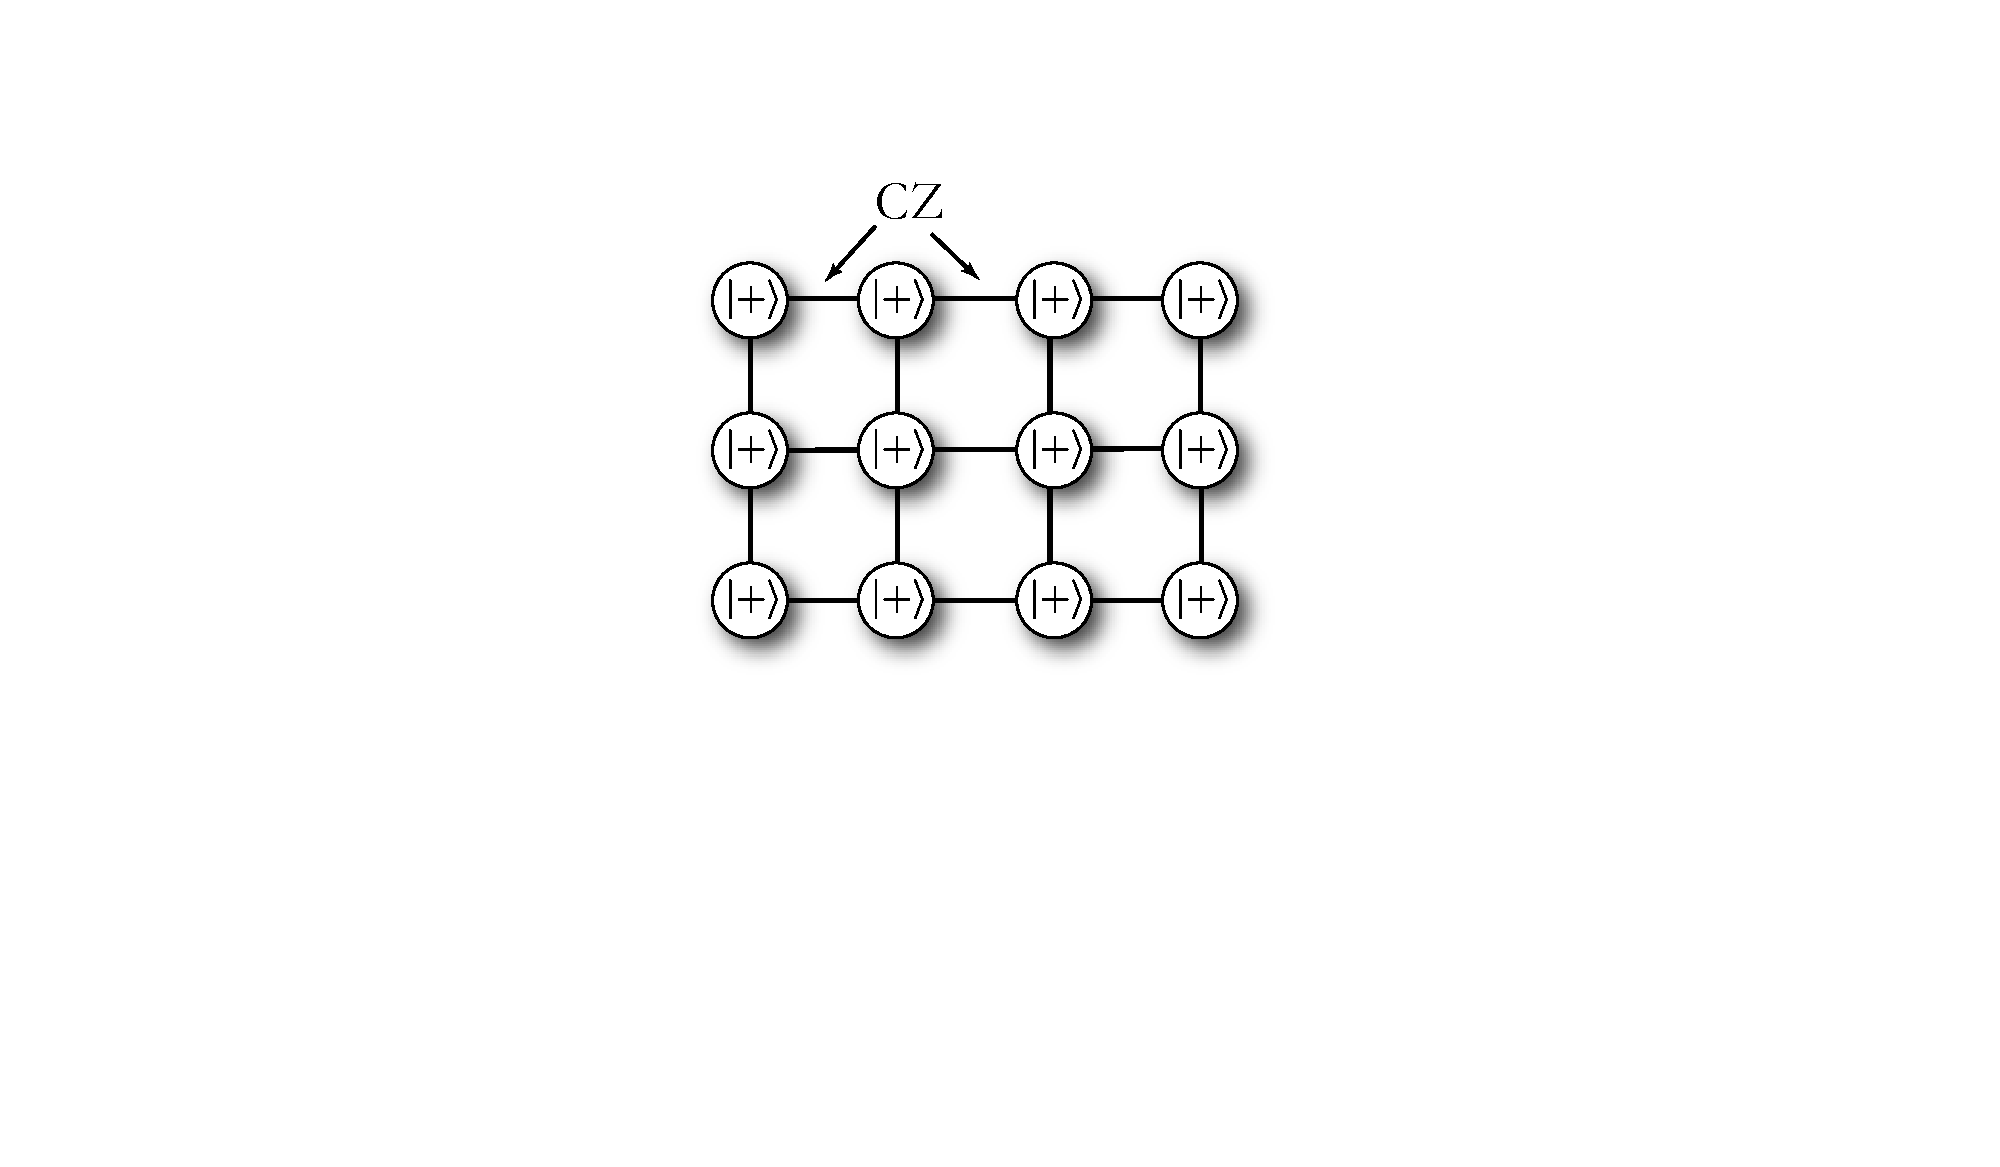
\includegraphics[width=0.6\columnwidth]{cluster_state}
\caption{The representation of cluster states as a graph. Vertices represent qubits initialised into the $\ket{+}$ state, while edges represent the application on CPHASE gates, the ordering of which is irrelevant.} \label{fig:cluster}	
\end{figure}

Unfortunately, implementing CPHASE gates using linear optics is complicated and highly non-deterministic. A major improvement upon this is to use fusion gates - rotated polarising beamsplitters, which implement projections onto the Bell basis. These operations fuse smaller cluster states, represented using polarisation encoding, into larger ones, consuming one (type-I fusion) or two (type-II fusion) photons in the process. These operations are shown in Fig.~\ref{fig:fusion}. Although these operations are non-deterministic with a success probability of $1/2$, they require only a single beamsplitter, already a major improvement over directly implementing CPHASE gates. Furthermore, unlike CPHASE gates, fusion operations require only high Hong-Ou-Mandel visibility, rather than the Mach-Zehnder stability required within existing CPHASE gate implementations, a major experimental simplification.

Although these gates are non-deterministic and consume qubits, strategies have been described for efficiently preparing arbitrarily large cluster states of arbitrary topology, and using far fewer optical elements than by directly employing CPHASE gates.

\begin{figure}[!htb]
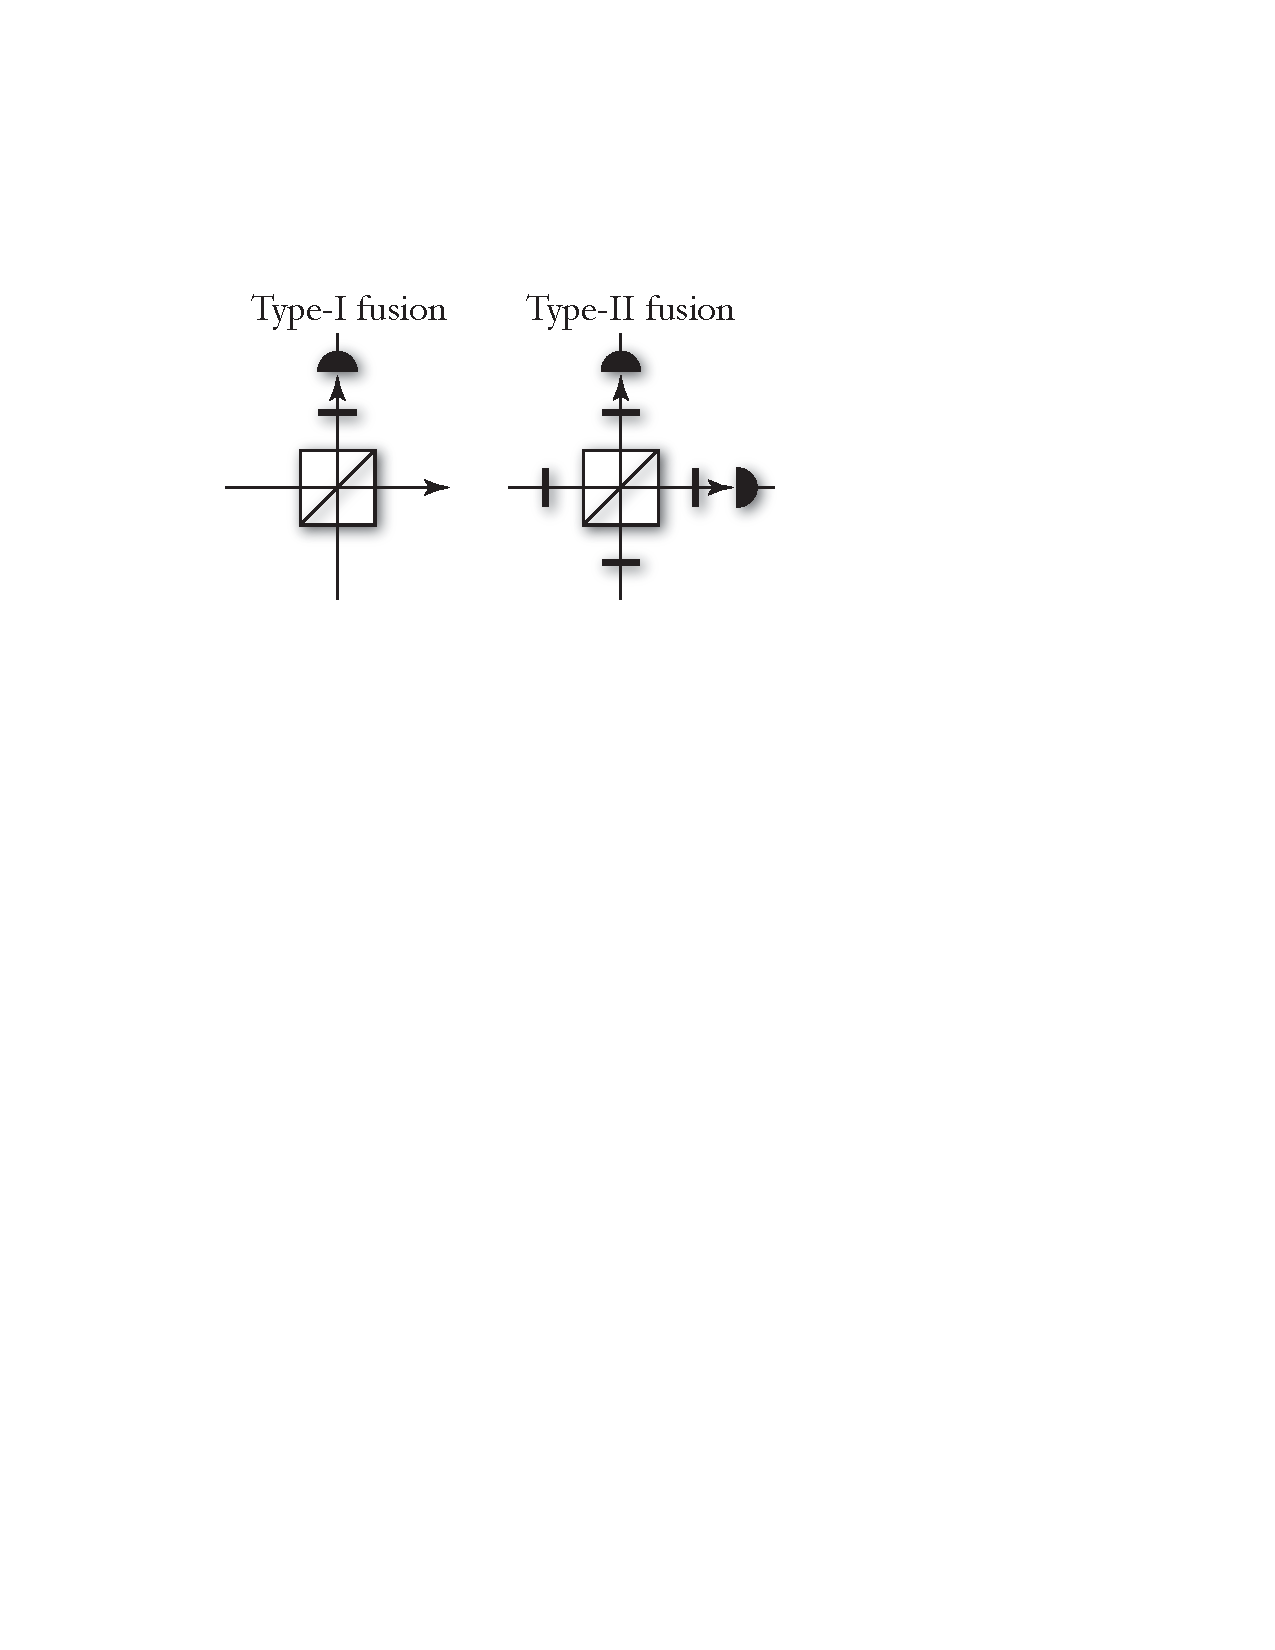
\includegraphics[width=0.7\columnwidth]{fusion}
\caption{Fusion gates for joining smaller cluster states into larger ones. Both require only a single polarising beamsplitter, and waveplates. The type-I and -II fusion gates consume 1 or 2 qubits (photons) respectively, creating an edge between the remaining graphs. The type-I gate consumes one fewer photon, but requires number-resolved detection on the detected mode. The type-II gate requires only on/off photodetection, but consumes an additional photon. Thus, the type-I gate can be employed to fuse two Bell pairs into a 3-qubit cluster state, whereas the type-II gate will only grow clusters when beginning with at least 3 qubits per cluster.} \label{fig:fusion}	
\end{figure}

\subsection{Linear optics networks}

Numerous experimental implementations of various linear optics protocols have been demonstrated, using a variety of architectures. The main contenders considered to date are: bulk-optics; waveguides; and time-bin encoding.

\subsubsection{Bulk-optics}

The early implementations of linear optics protocols relied on bulk-optics implementations, in which a circuit is decomposed into a discrete arrangement of optical components, specifically beamsplitters and phase-shifters. This corresponds to a direct implementation of the Reck \emph{et al.} decomposition shown in Fig.~\ref{fig:Reck}, or subsequent alternate decompositions.

Although this approach is effective and conceptually straightforward, it is highly impractical for large interferometers. For example, the implementation of a 100-mode interferometer requires on the order of 10,000 discrete optical elements, which must all be simultaneously aligned with interferometric stability, a highly experimentally challenging problem, not to mention incredibly physically large.

\subsubsection{Waveguides}

Alternately, integrated waveguide devices can be employed to implement identical decompositions by etching the modes into paths in an optical chip, where evanescent coupling between closely neighbouring modes implements beamsplitter operations. Such devices are extremely compact, allowing the miniaturisation of large numbers of optical elements. Importantly, such devices are extremely optically stable, mitigating the need for any kind of dynamic stabilisation

\subsubsection{Time-bins}\label{sec:timebins}

Using time-bin encoding of optical qubits, the obvious question is how to perform operations upon them. In \cite{bib:Motes14}, a dual-loop architecture was presented for implementing arbitrary passive linear-optics on photonic pulse-trains, shown in Fig.~\ref{fig:FL_arch}.

\begin{figure}[!htb]
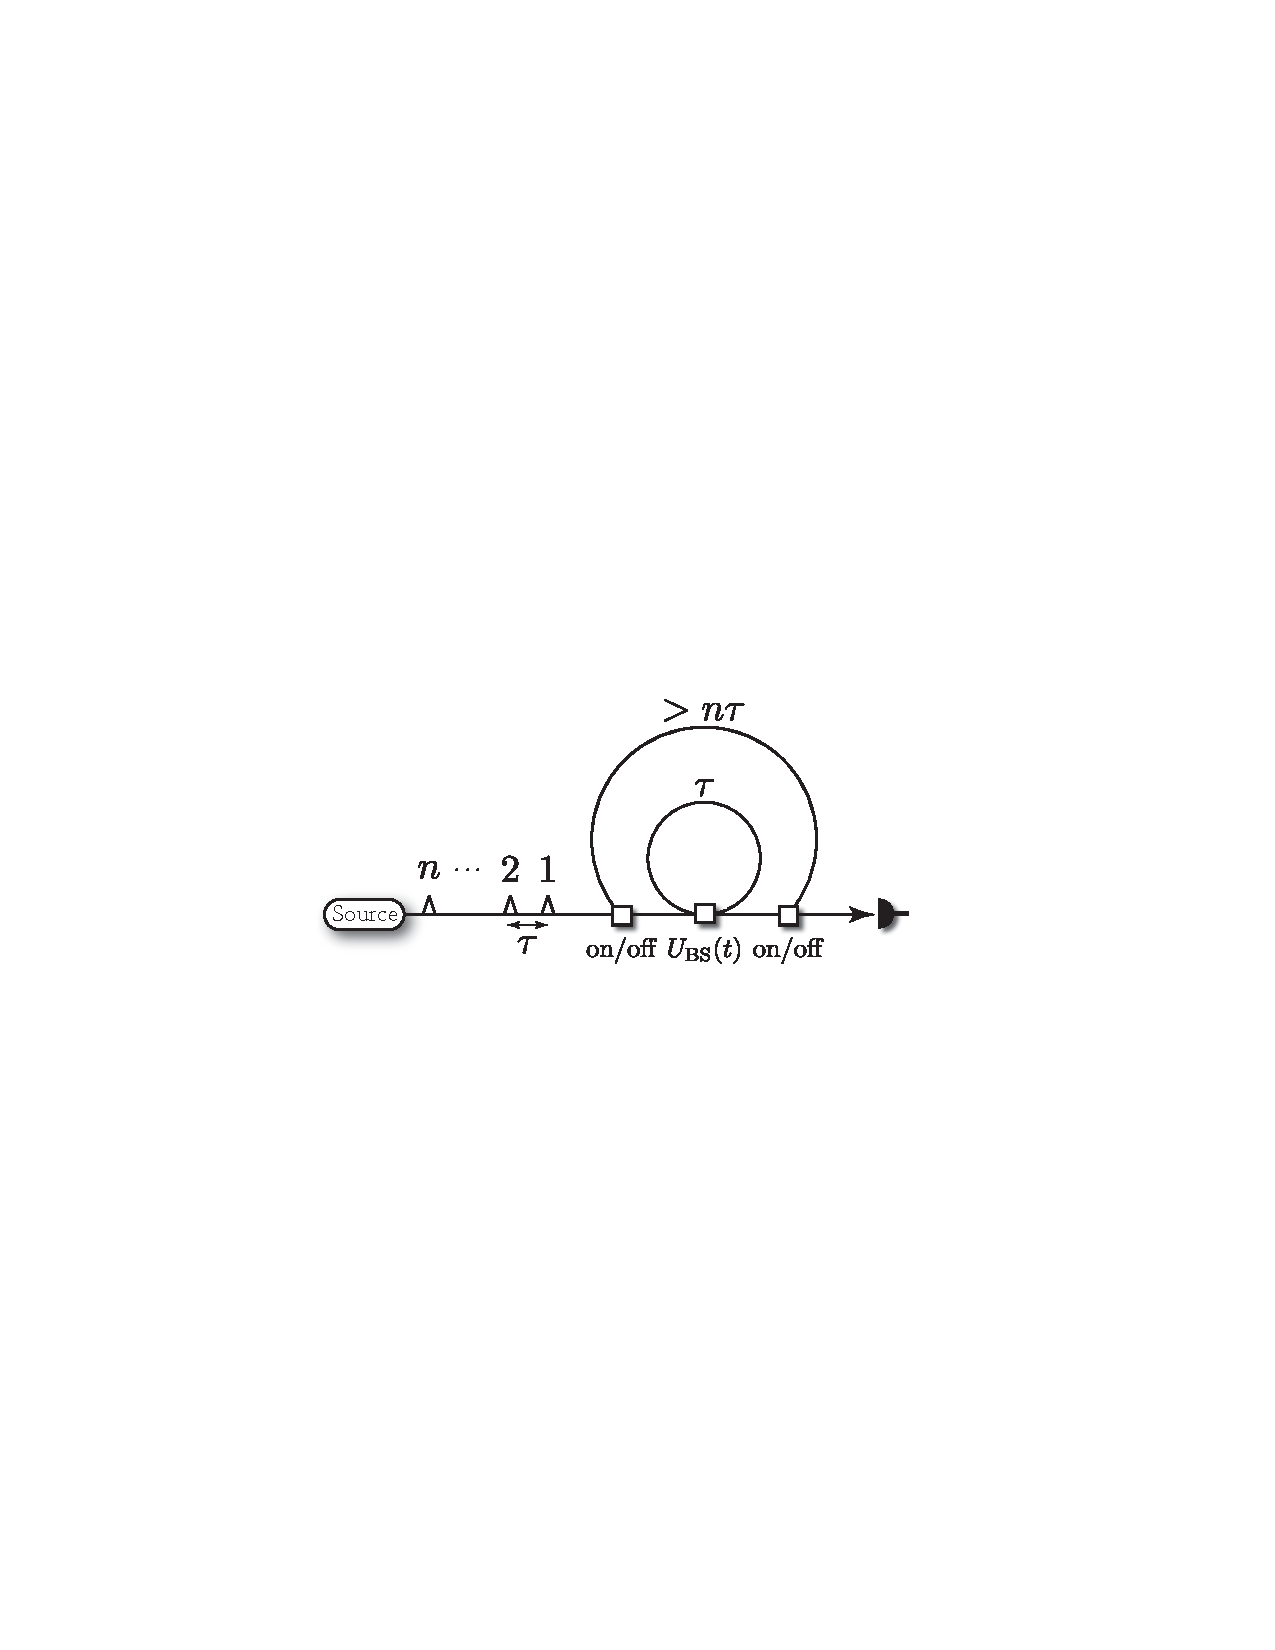
\includegraphics[width=\columnwidth]{full_architecture}
\caption{A fibre-loop architecture for implementing arbitrary linear optics operations upon a time-bin-encoded pulse-train. The source prepares the temporally encoded pulse-train, with time-bin separation $\tau$. The pulse-train then enters a dual-loop configuration. The inner loop has length exactly $\tau$, while the outer one has length $>n\tau$ ($n$ is the number of optical modes). The architecture is controlled via three dynamically controlled beamsplitters. The first and last need only be on/off switches, whose sole purpose is to couple in the prepared pulse-train, keep it within the outer loop for the required duration, and then couple out of the outer loop, yielding the transformed pulse-train. The central beamsplitter must be able to implement arbitrary classically-controlled beamsplitter operations.} \label{fig:FL_arch}	
\end{figure}

The architecture is frugal in its use of optical components, requiring only three dynamic beamsplitters, and several lengths of fibre. The beauty of this architecture is that the experimental requirements do not increase with the number of optical modes. The only parameter that scales with the number of optical modes is the outer loop, which must be at least long enough to house the entire time-bin-encoded pulse-train. Note, however, that the central beamsplitter must be controllable at sub-$\tau$ time-scales, so as to enable each temporal mode to be addressed individually, which is technically challenging.

The workings of the scheme can be thought of as follows: the inner loop allows arbitrary beamsplitter operations between neighbouring time-bins; the outer loop does nothing interferometric, but rather enables the pulse-train to undergo as many applications of the inner loops as necessary. It then follows that this scheme is universal for linear optics, as a sufficient number of beamsplitter operations between neighbouring modes enables universal decompositions, using for example, the Reck \emph{et al.} decomposition described earlier.

As a simple example of how such time-bin encoding maps to other encodings, in Fig.~\ref{fig:PBS_TB} we show the isomorphism between the polarising beamsplitter operation and a pairwise temporal beamsplitter operation. This implies a direct mapping for implementing cluster state preparation within the time-bin scheme.

\begin{figure}[!htb]
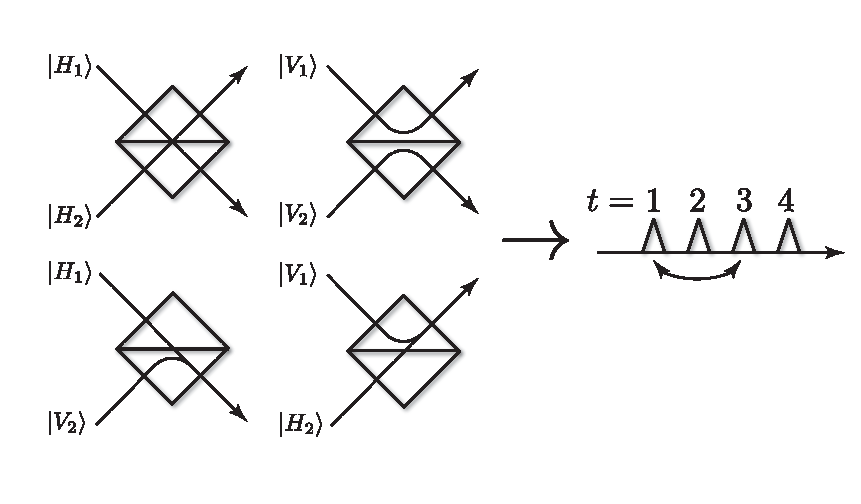
\includegraphics[width=0.7\columnwidth]{PBS_TB}
\caption{Mapping between two polarisation-encoded qubits undergoing a polarising beamsplitter (PBS) operation, and its equivalent representation using 4 time-bins in a pulse-train. The PBS completely reflects (transmits) the vertical (horizontal) polarisations. The evolution of the four logical basis states, and their respective outputs, are shown explicitly. Writing out this PBS transformation in matrix form yields a permutation. Taking this permutation and relabelling the modes, we obtain the time-bin transformation shown underneath -- a simple swap of two of the four time-bins.} \label{fig:PBS_TB}	
\end{figure}

The above description applies to passive linear optics, which is sufficient for protocols such as {\sc BosonSampling}, but insufficient for universal optical quantum computation, which requires the addition of ancillary states, and measurement with fast-feedforward. To address this, it was shown in \cite{Rohde} that by dynamically preparing ancillary pulse-trains (from the already-existing source), classically controlled by time-resolved measurements at the output, and changing the switching sequence, we can effectively couple in and out arbitrary subsets of the optical modes, enabling partial measurements to be implemented.

\subsection{Photodetection}

Broadly speaking, there are two main classes of photodetectors: number resolved, and non-number-resolved (also referred to as bucket, or on/off) detectors. As the names suggest, these detectors are able to measure photon-number, or merely the presence or absence of photons. They are described by the measurement projectors,
\begin{align}
\hat\Pi_n &= \ket{n}\bra{n}, \nonumber \\
\hat\Pi_\text{off} &= \hat\Pi_0, \nonumber \\
\hat\Pi_\text{on} &= \hat{I} - \hat\Pi_\text{on},	
\end{align}
respectively.

The dominant challenge facing the experimental implementation of both types of detectors is inefficiency, which results in higher photon-number being confused as having lower photon-number. In some protocols, such as type-II fusion, which relies on coincidence detection, inefficiency is not problematic. However, in most applications, including type-I fusion, this is highly problematic as photon-number confusion results in decoherence via projecting onto the wrong photon-number, unknown to the observer.

\comment{What are the different technologies}

\section{Applications for linear optics interferometry}

\subsection{Linear optics quantum computation}

\subsection{Boson-sampling}

\subsection{Quantum metrology}

\comment{Discuss NOON states - Heisenberg limited}

\comment{Discuss MORDOR scheme}

\section{Conclusion}

Linear optics interferometry has become a leading contender for the implementation of quantum information processing protocols. The preparation, manipulation and measurement of photonic quantum information has become mainstream and widely employed, with impressive experimental accuracies.

We have discussed the various ways in which quantum information can be represented photonically, how they can be manipulated and detected, and some of their leading applications.

Although there are countless physical architectures for the implementation of quantum information processing, and it is far from certain which will win `the quantum race for supremacy', optics will always find a home as the only contender for applications involving quantum communication. For this reason, the future of linear optics interferometry is a bright one, which will find inevitable applicability in the future quantum world.

%
% Acknowledgments
%

\begin{acknowledgments}
P.P.R. is funded by an ARC Future Fellowship (project FT160100397).
\end{acknowledgments}

%
% Bibliography
%

\bibliography{paper}

\end{document}
